\documentclass[a4paper]{article}
\usepackage{listings}
\usepackage{graphicx}
\graphicspath{ {../images/} }
\addtolength{\hoffset}{-2.25cm}
\addtolength{\textwidth}{4.5cm}
\addtolength{\voffset}{-3.25cm}
\addtolength{\textheight}{5cm}
\setlength{\parskip}{0pt}
\setlength{\parindent}{0in}

%----------------------------------------------------------------------------------------
%	PACKAGES AND OTHER DOCUMENT CONFIGURATIONS
%----------------------------------------------------------------------------------------

\usepackage{blindtext} % Package to generate dummy text
\usepackage{charter} % Use the Charter font
\usepackage[utf8]{inputenc} % Use UTF-8 encoding
\usepackage{microtype} % Slightly tweak font spacing for aesthetics
\usepackage[english, ngerman]{babel} % Language hyphenation and typographical rules
\usepackage{amsthm, amsmath, amssymb} % Mathematical typesetting
\usepackage{float} % Improved interface for floating objects
\usepackage[final, colorlinks = true, 
            linkcolor = black, 
            citecolor = black]{hyperref} % For hyperlinks in the PDF
\usepackage{graphicx, multicol} % Enhanced support for graphics
\usepackage{xcolor} % Driver-independent color extensions
\usepackage{marvosym, wasysym} % More symbols
\usepackage{rotating} % Rotation tools
\usepackage{censor} % Facilities for controlling restricted text
\usepackage{listing} % Environment for non-formatted code, !uses style file!
\usepackage{pseudocode} % Environment for specifying algorithms in a natural way
%\usepackage{style/avm} % Environment for f-structures, !uses style file!
\usepackage{booktabs} % Enhances quality of tables
\usepackage{tikz-qtree} % Easy tree drawing tool
\tikzset{every tree node/.style={align=center,anchor=north},
         level distance=2cm} % Configuration for q-trees
%\usepackage{style/btree} % Configuration for b-trees and b+-trees, !uses style file!
\usepackage[backend=biber,style=numeric,
            sorting=nyt]{biblatex} % Complete reimplementation of bibliographic facilities
\addbibresource{ecl.bib}
\usepackage{csquotes} % Context sensitive quotation facilities
\usepackage[yyyymmdd]{datetime} % Uses YEAR-MONTH-DAY format for dates
\renewcommand{\dateseparator}{-} % Sets dateseparator to '-'
\usepackage{fancyhdr} % Headers and footers
\pagestyle{fancy} % All pages have headers and footers
\fancyhead{}\renewcommand{\headrulewidth}{0pt} % Blank out the default header
\fancyfoot[L]{} % Custom footer text
\fancyfoot[C]{} % Custom footer text
\fancyfoot[R]{\thepage} % Custom footer text
\newcommand{\note}[1]{\marginpar{\scriptsize \textcolor{red}{#1}}} % Enables comments in red on margin

%----------------------------------------------------------------------------------------

\begin{document}

%-------------------------------
%	TITLE SECTION
%-------------------------------

\fancyhead[C]{}
\hrule \medskip % Upper rule
\begin{minipage}{0.295\textwidth} 
\raggedright
\footnotesize
Taten H. Knight \hfill\\   
L30052460\hfill\\
knight.taten@gmail.com
\end{minipage}
\begin{minipage}{0.4\textwidth} 
\centering 
\large 
Homework Assignment 1\\ 
\normalsize 
General Knowledge on Computer Science\\ 
\end{minipage}
\begin{minipage}{0.295\textwidth} 
\raggedleft
\today\hfill\\
\end{minipage}
\medskip\hrule 
\bigskip

%-------------------------------
%	CONTENTS
%-------------------------------

\section{Inquiry 1}
Week 1 of Research in Computer Science covered three core subjects: algorithm analysis, algorithm correctness, and software verification. These subjects are both fundamental to the study of computer science and remain relevant in the present and future progress of the field. I will briefly review the related literature for each topic and finish with a short summary and their relationship to each other and to the broader field of computer science.

\subsection{Algorithm Analysis}
Algorithm analysis is the process of examining an algorithm and determining its overall efficiency in memory and time, most commonly described in terms of \emph{complexity}. For some function $f(x)$ what is the complexity $C$ w.r.t. $x$. The most commonly used descriptor of complexity is big O notation, which describes the known worst possible behavior of the algorithm with respect to the input. $\theta$ notation describes the asymptotic behavior of the algorithm. For example, for the following 'algorithm' has a theta time complexity of $\theta(A)$ because the time it takes to run is proportional to the value of A:
\begin{lstlisting}
A = 10
for a in [1:A]:
  print(a)
\end{lstlisting}
Space (memory) describes the memory taken up during the execution of the algorithm. The previous algorithm has space complexity of $O(N)$ because each element of the array must be stored and printed. There are others ways to describe the complexity of algorithms that have more strict criteria or describe other conditions, but the main point of algorithm analysis is to determine if use of the algorithm is viable in its environment, or if we need to use a more efficient solution to meet our constraints.

\subsection{Algorithm Correctness}
Determining algorithm correctness is determining if a given algorithm yields the correct results across all possible inputs, including handling invalid inputs appropriately. Correctness is paramount in safety-critical systems and important in all others to guarantee functionality. Absolute correctness is determined via the use of formal mathematical proofs. At the low level algorithm level this can be simple, but correctness is also needed at a high level for large software systems. To do this we can apply these proofs at a high level using software verification techniques.

\subsection{Software Verification}
Software verification is the process of determining whether software functions as intended. There are different standards for correctness and different methods of verifying the software. Verification can fall into three categories: peer review, testing, and formal methods. Peer review requires individuals manually reviewing code that has not been run, and only catches approximately 60\% (median) of errors. There is testing which involves running human written tests for correct outcomes, and requires a large chunk of development time being devoted to writing the tests. Lastly there is formal verification, which uses formal mathematical methods to verify that the software only has outputs with the specified criteria. Although it is very intensive, the verification method is generally reusable after it has been created once for a given software system and can save many man hours for repeated verification. It can also provide better coverage, though it suffers the same drawbacks as other forms of verification; it cannot confirm the lack of errors, only the presence of them.

\subsection{Summary}
When developing software, the goal is to create software that performs the intended function, is correct (in that it responds appropriately to inputs with correct outputs), and is efficient enough to be used in a production environment. We can accomplish these goals through algorithm analysis, determining correctness on the individual algorithm level, and verifying software systems via peer review, testing, and formal verification. Although formal verification has not been easily achievable until relatively recently, some major companies such as Dassault-Aviation are using formal verification, testing, and peer-review in verifying portions of safety-critical systems, which indicates a shift away from past paradigms. This shift can result in better coverage and more long-term savings over a software development cycle.

\section{Inquiry 2}
\emph{Software Verification: Testing vs. Model Checking} by D. Beyer and T. Lemberger, compares the current viability of automatic software testing against that of automatic software model checking. They concluded that software model checking is now mature enough to surpass automatic software testing in finding bugs in a program by comparing the results of both methods (six testing tools and four model checkers) on 5693 C programs. They also stress that testing should not be removed completely, but that  model checking can outperform testing in some circumstances, and that a combination of methods can yield better overall results.

\subsection{Definitions}
\emph{Software testing} is when a verification program is given a set of specifications and a wide set of input values, and we verify that the specifications hold across the test inputs. \emph{Model Checking} explores the entire state space of the software and looks for violations of the given specification. Note that because the potential states of a program are essentially infinite we use an abstraction that simplifies or narrows the state space while still providing good coverage. ''A \emph{violation witness} is an automaton that describes a set of paths through the program that contain a specification violation.''

\subsection{Methods}
The study took four separate model checkers and 6 automatic software testers that each operated off of different principles and ran them against the 5693 separate C programs. They then took the results of these runs (the found bugs) and verified that they were correct using violation witnesses. They accomplished this by building a unifying framework for test best falsification that formats the source code of the C program, runs the test generator, extracts tests vectors, and checks if the tests cases exposed a bug. 

\subsection{Results}
The results can be summarized by looking at the table from the study shown below:
\linebreak
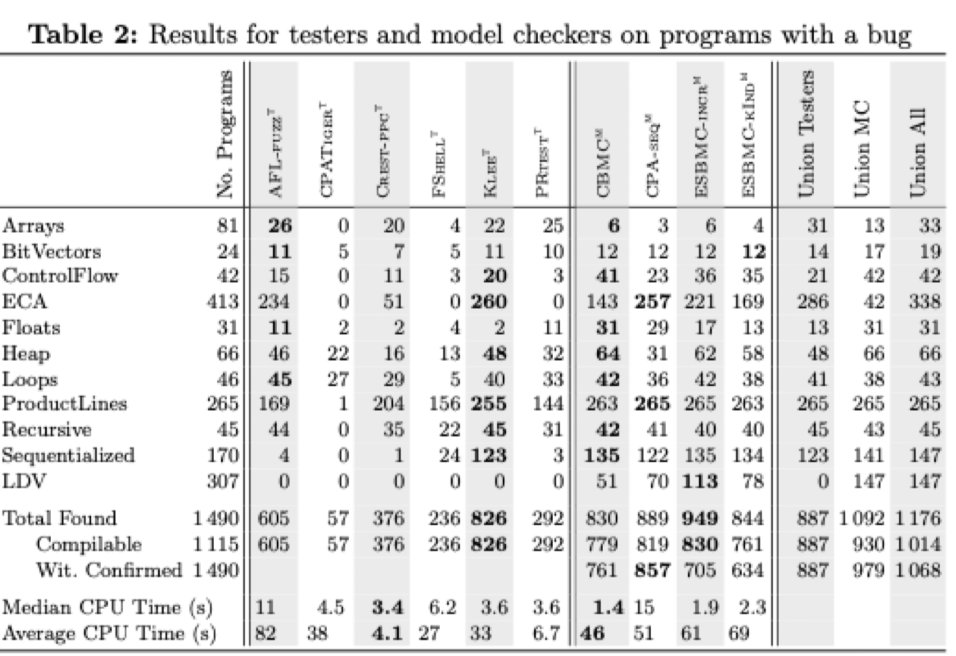
\includegraphics{results}
\linebreak
We can see that all of the model checkers outperform the testers on total bugs found, and another result shows that the model checkers also have lower CPU times across the board. The only comparable tester is the KLEE in both CPU time and bugs found. Interestingly, each of the tests fail to catch different bugs, and the Union All column shows that the most bugs can be found by applying all model checkers and tests.

\subsection{Conclusion}
Based on the above results we see that if you are only able to choose a single verification method, a model checker is the best choice for finding the largest number of bugs as efficiently as possible. If, however, the goal is to find as many bugs as possible, combining multiple model checkers and testers will yield the highest number of bugs.

\end{document}
